\section{Systembeskrivelse}
Denne sektion vil beskrive hvordan systemet sat op. samt hvilke chips og boards der er udleveret.
Til projektet er der anvendt det tildelte pan tilt system som har påmonteret et protection board, 2 hall sensorer 2 h-broer og 2 motorer, der sidder på hhv pan og tilt.\\
Til at styre denne opstilling er der udleveret èt stk Field Programmable Gate Array (FPGA) og èn Micro processor unit (MPU).
\\

\subsection{Fysiske begrænsninger}
XXXX Daniel skriver vel det her :p

\subsection{Micro Processor Unit}
Det udleverede Launchpad board som er et EK-TM4C123GXL board, er fra Texas Instruments, den har en påmonteret MPU som er af modellen TM4C123GH6PM, denne er en Arm Cortex M4 chip \cite{TM4C123GH6PMDatasheet}.\\
Launchpad boardet får strøm gennem micro usb porten som sidder i øverste venstre hjørne som ses på figur \ref{fig:TivaLaunchPad}.\\
Micro usb porten bruges samtidig til at programmere boarded ved hjælp af et Integrated development environment (IDE) til dette projekt blev Code Composer Studio \textsuperscript{\texttrademark} anvendt som er Texas Instruments egen IDE.

\begin{figure}[!ht]
	\begin{center}
		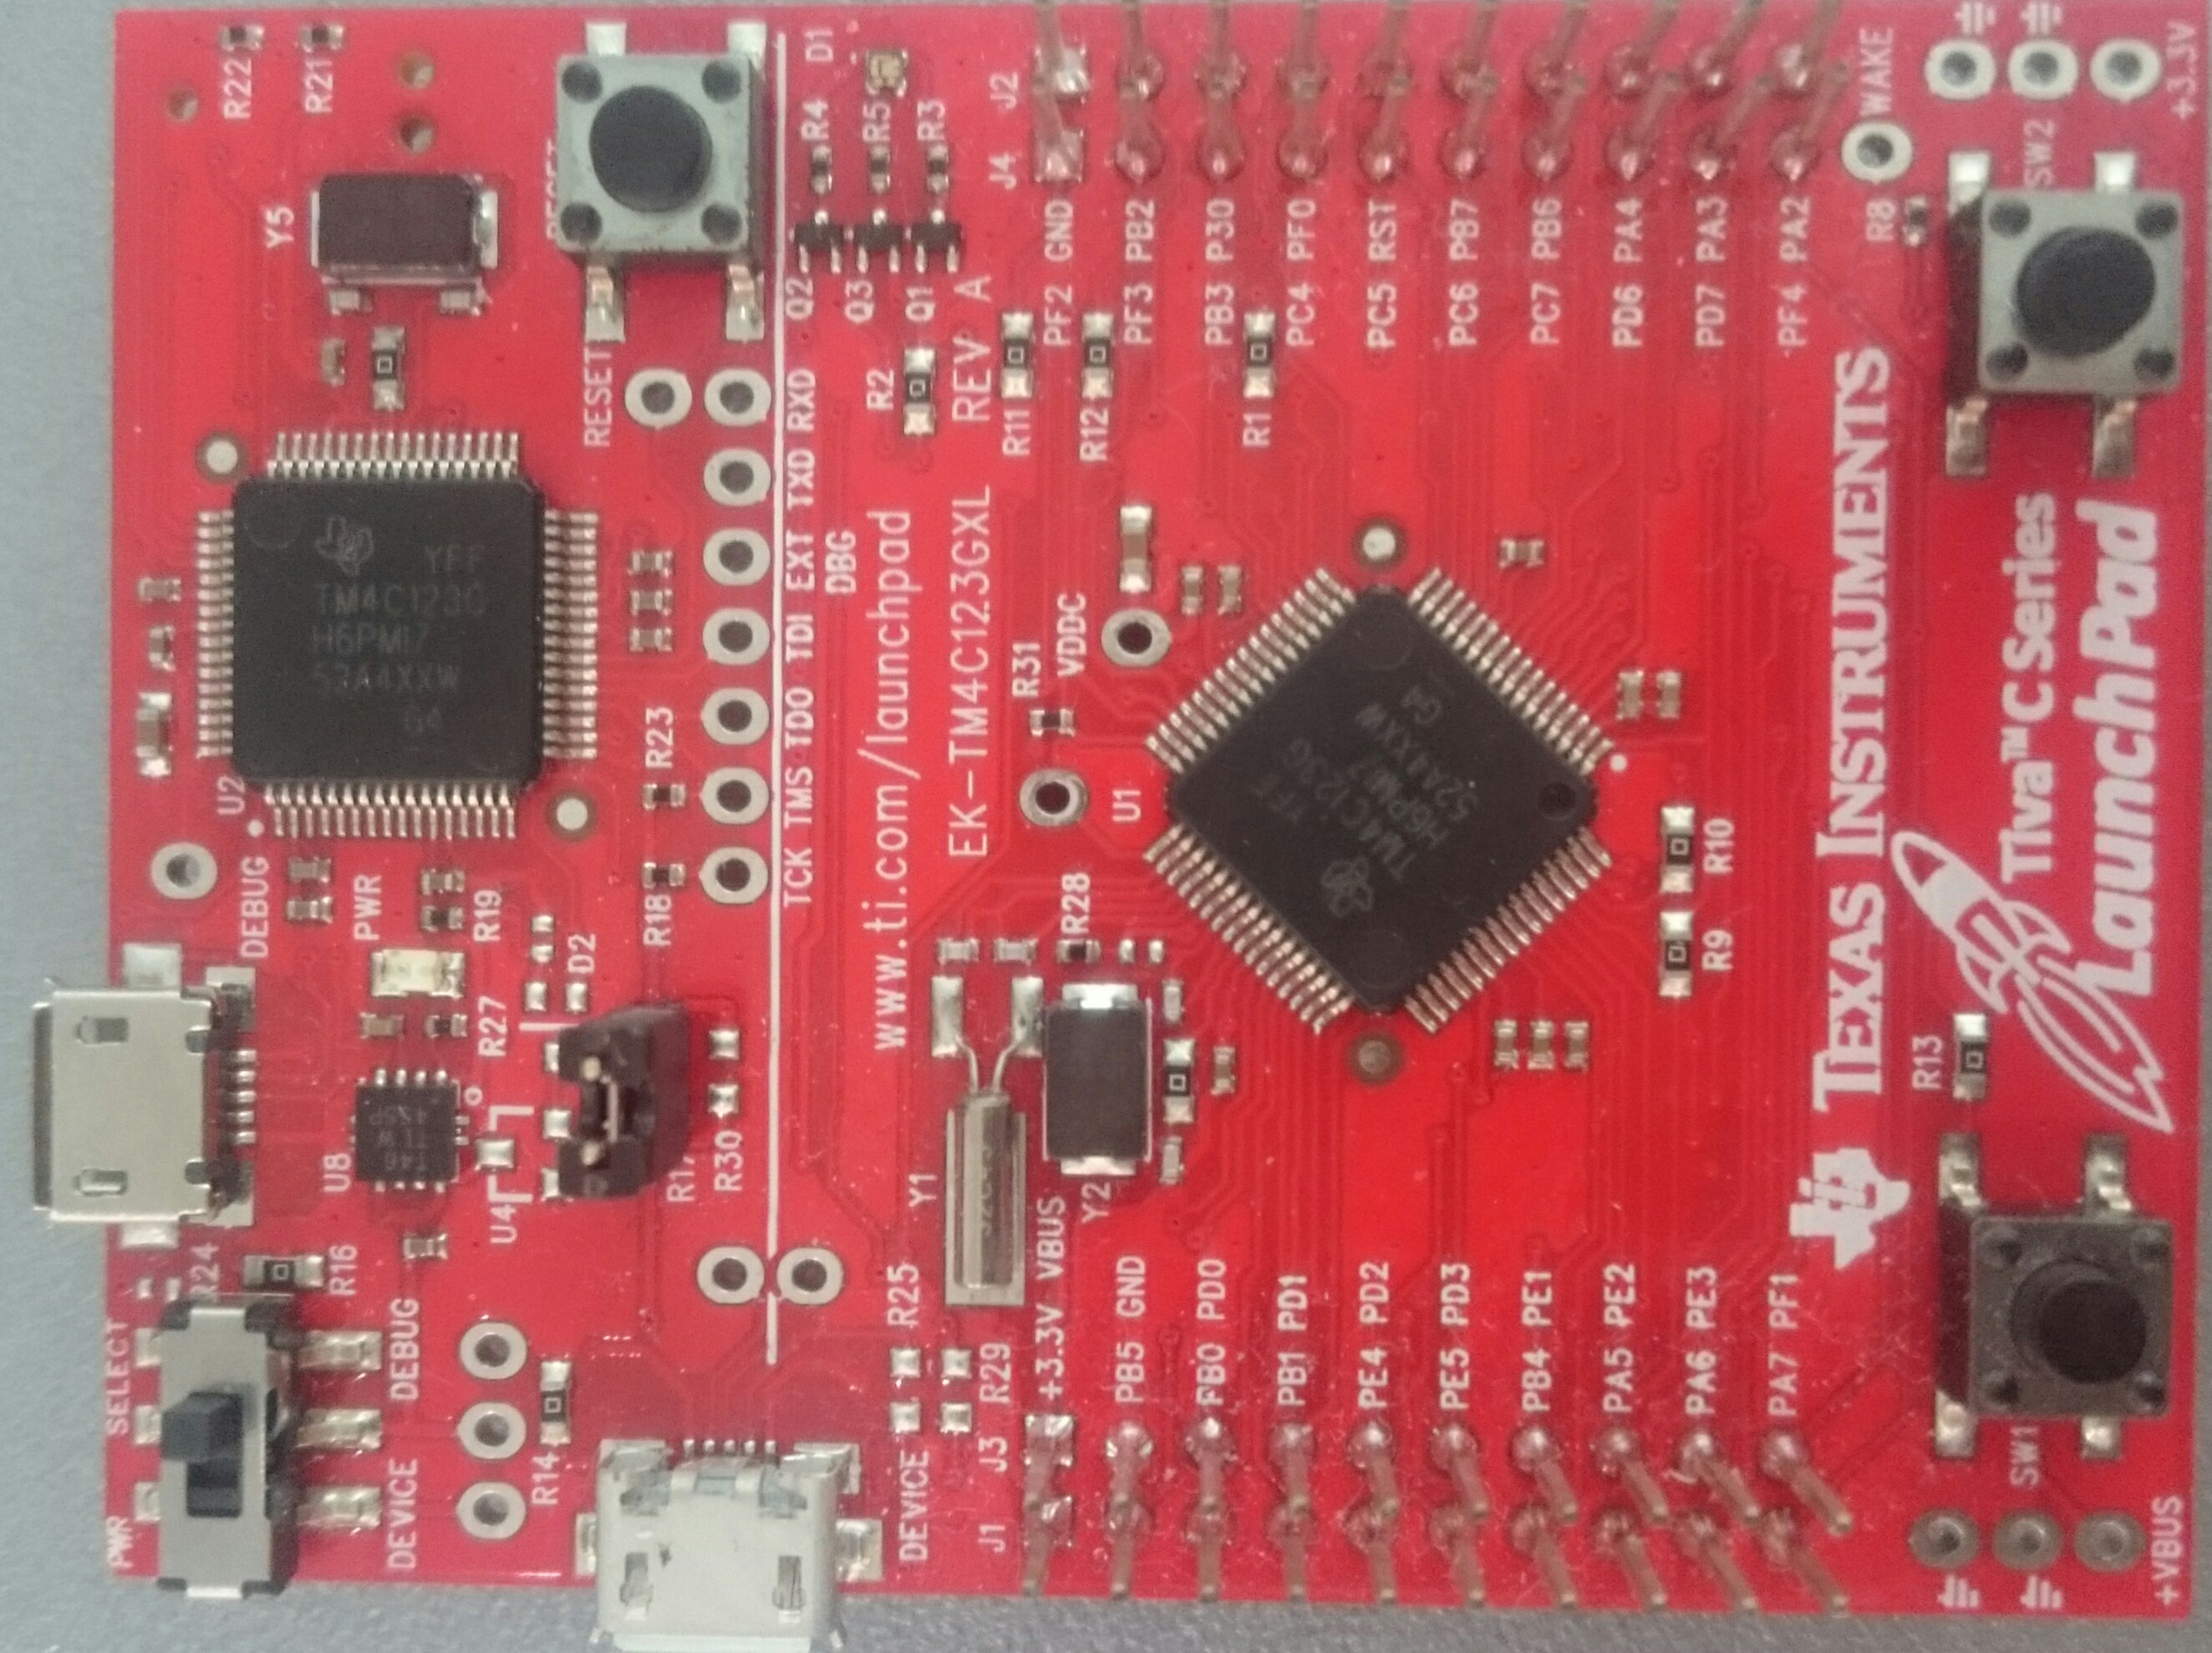
\includegraphics[scale=0.1, angle =270]{Billeder/TivaLaunchPad.JPG}
	\end{center}
\caption{Tiva\textsuperscript{\texttrademark} Launchpad boardet med den tilføjede TM4C123GH6PM arm cortex M4 Micro Processor Unit}
\label{fig:TivaLaunchPad}
\end{figure}

Launchpad boarded kan tilføjes til et embedded programmerings board som blev udleveret i starten af semesteret som inkluderer et keypad, et lcd og en drehimpulsgeber, samt en SPI udgang som anvendes til projektet, se figur \ref{fig:EMP_BOARD} og se vedlagt USB disk for at finde datablad, for mere information.

\begin{figure}[!ht]
	\begin{center}
		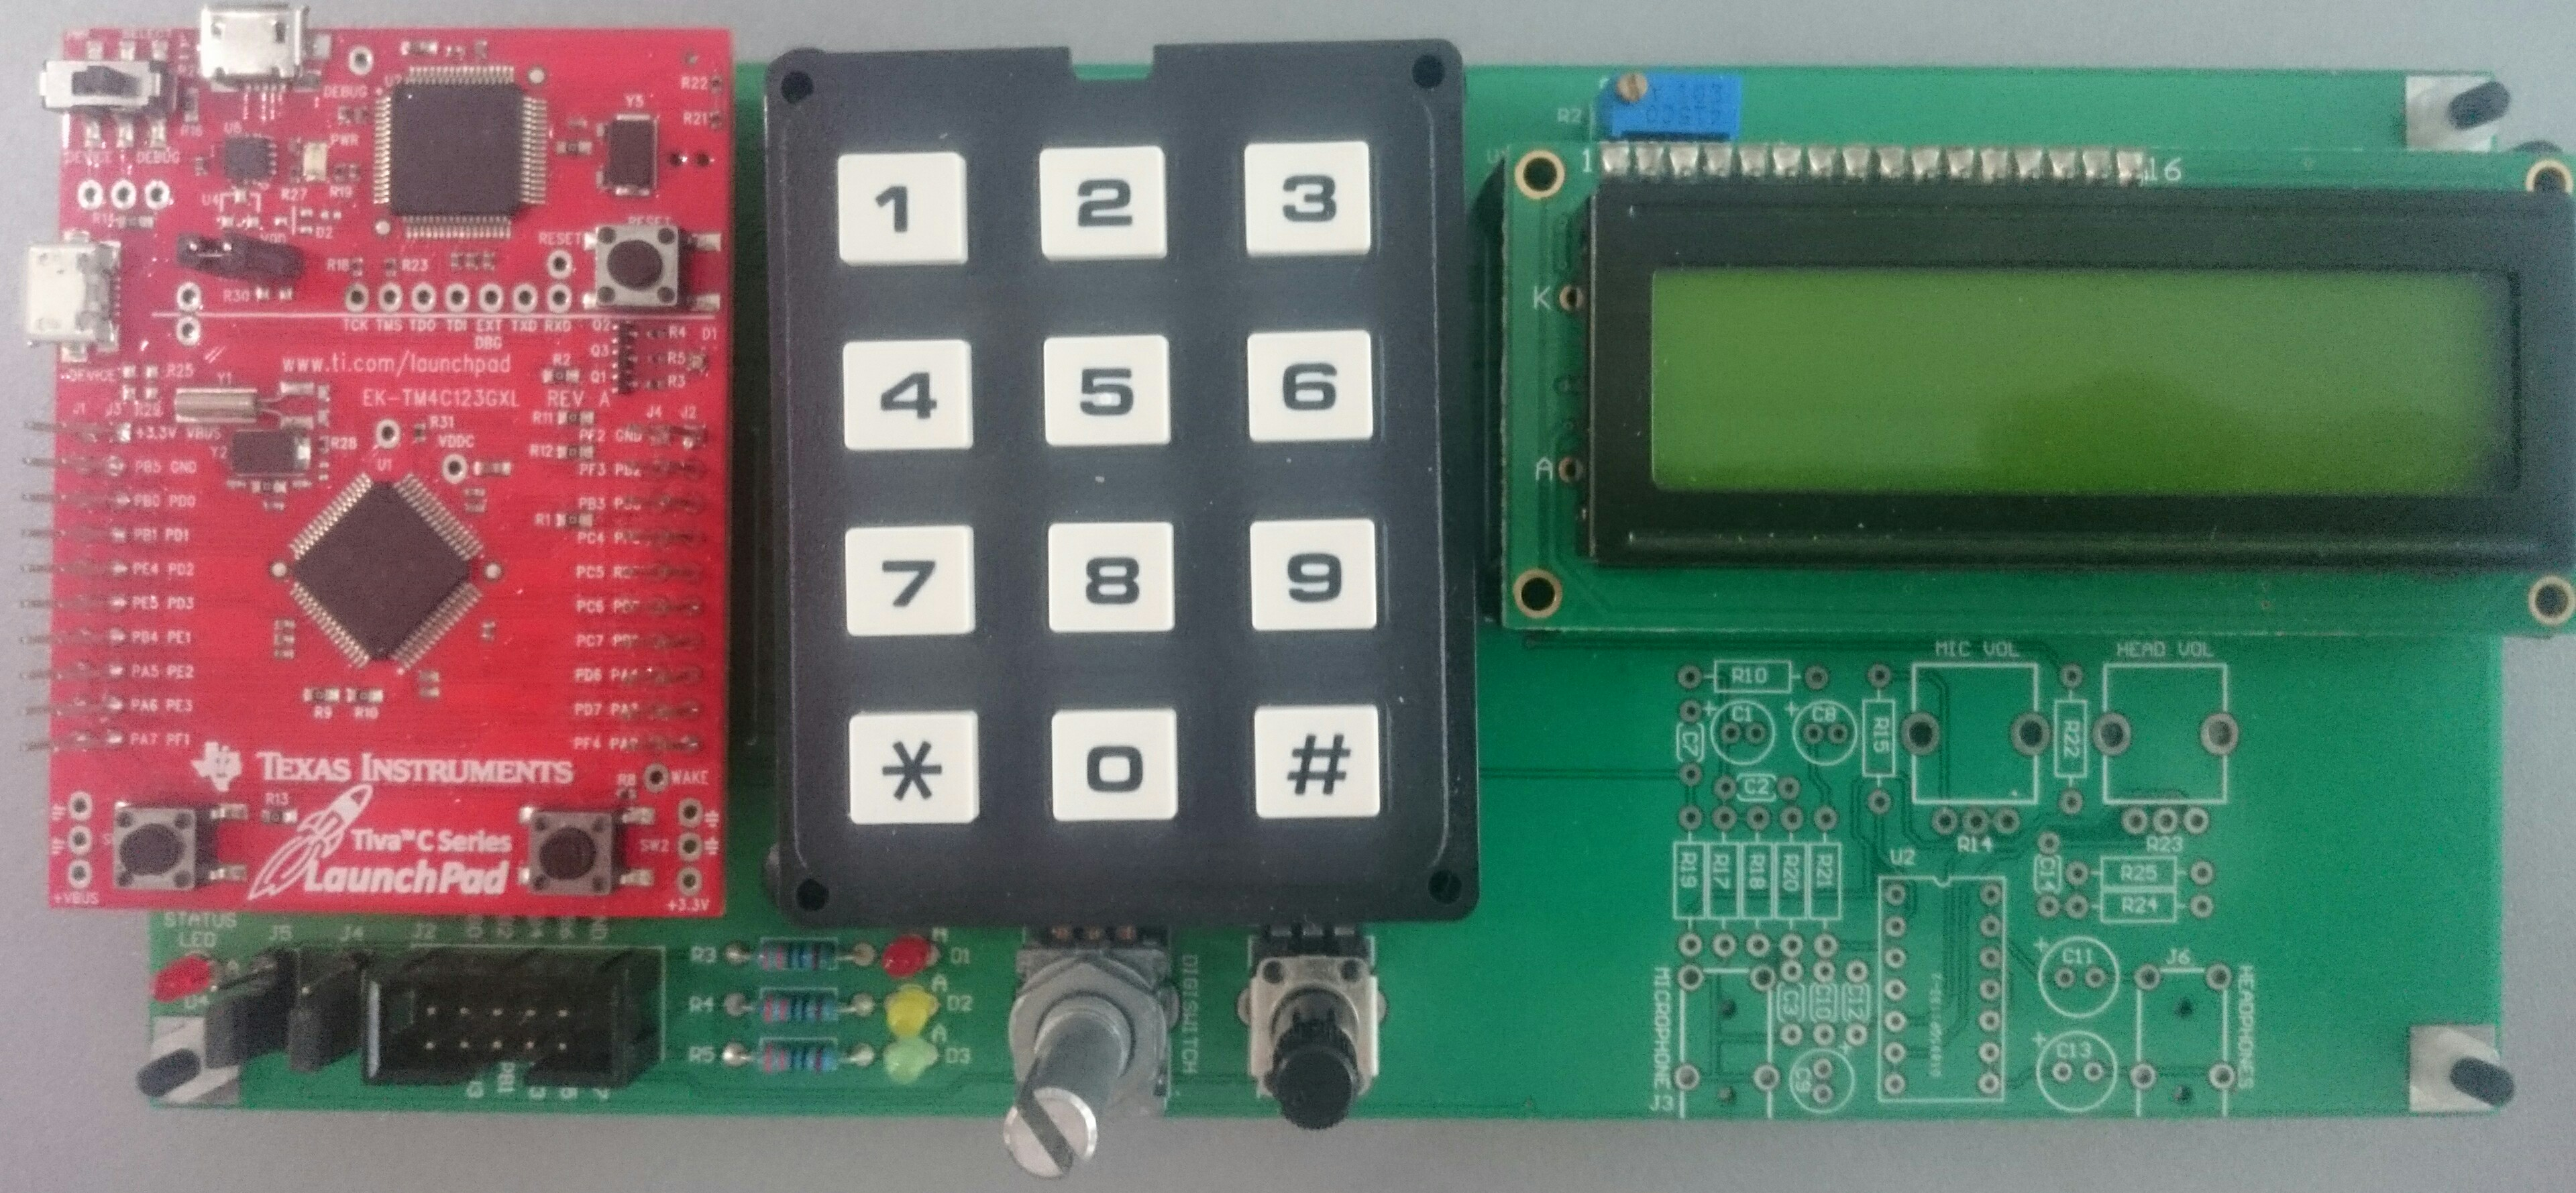
\includegraphics[scale=0.1, angle =0]{Billeder/EMP_BOARD.JPG}
	\end{center}
\caption{EMP Board med det tilføjede Launch pad board}
\label{fig:EMP_BOARD}
\end{figure}

\subsection{Field Programmable Gate Array}

Det udleverede board er en Nexys 2 af mærket Digilent, chippen som sidder på boardet er en Spartan-3E FPGA.

Nexys 2 boardet har 4x 7-segments displays, med 8 switches og 4 buttons. samtidig er der 3 porte som bliver brugt til projektet: JA,JC og JD, se figur \ref{fig:Nexys2Board} samt USB for at finde datablad og mere information.

\begin{figure}[!ht]
	\begin{center}
		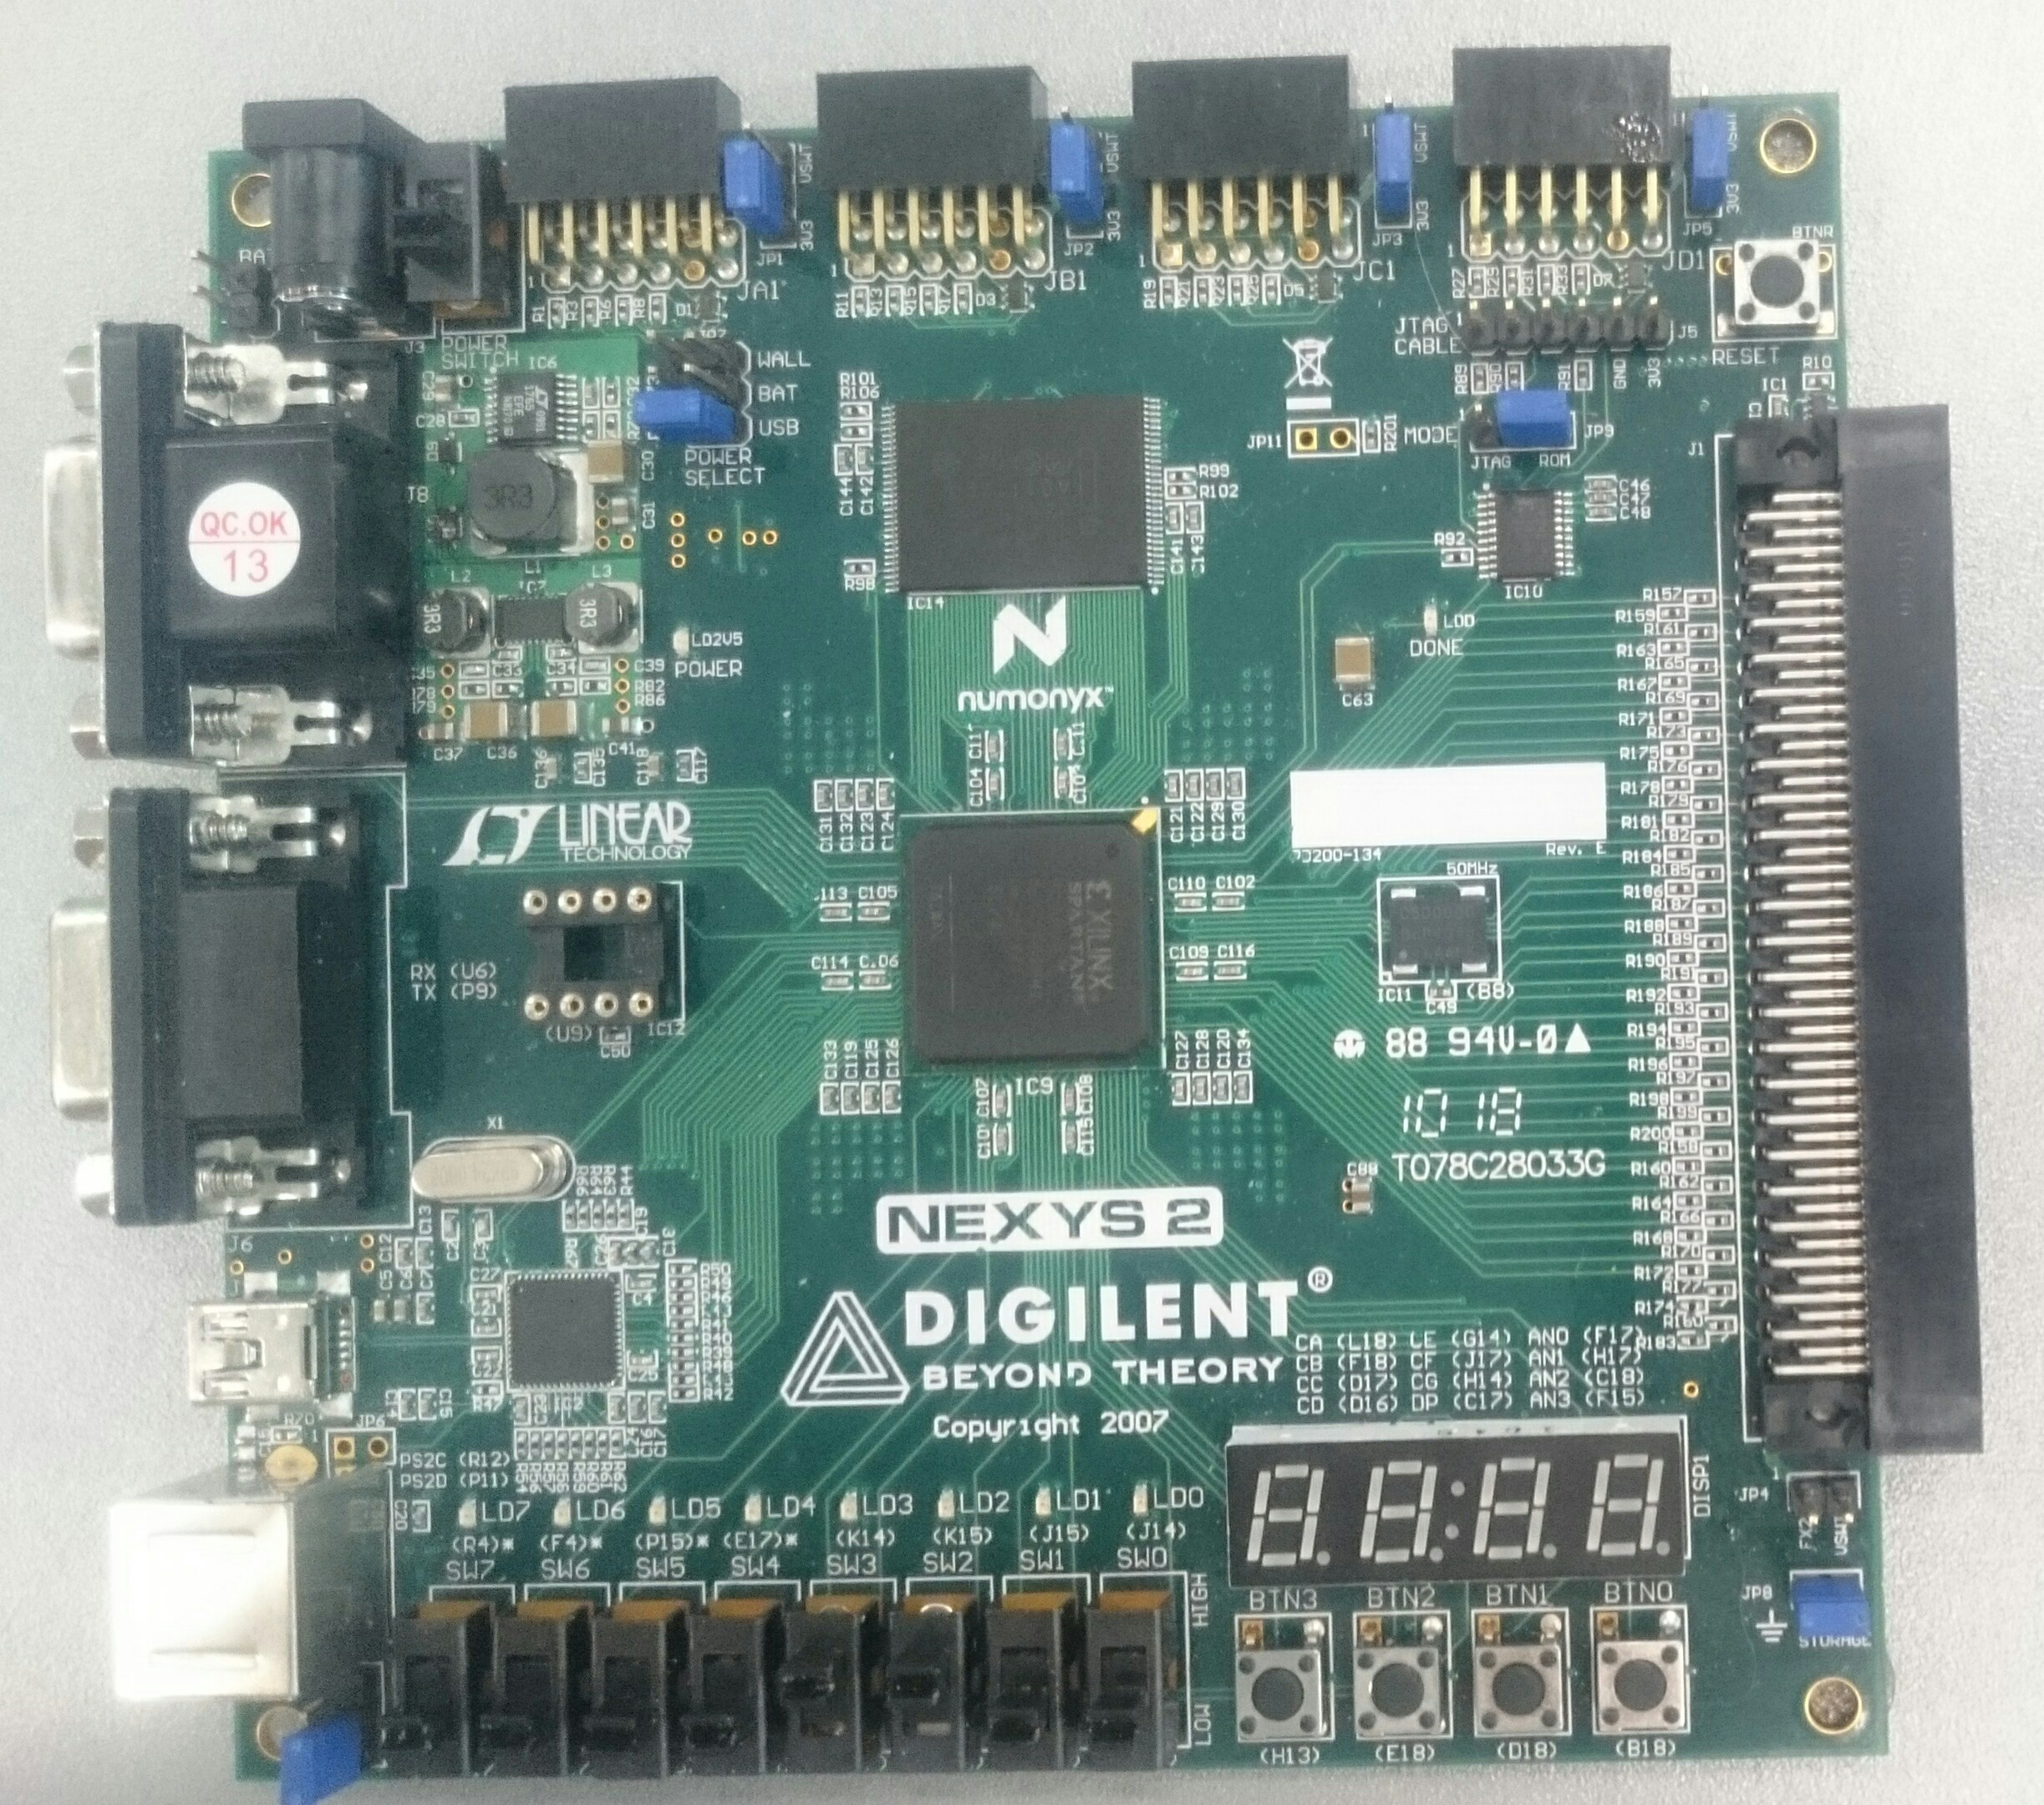
\includegraphics[scale=0.1, angle =0]{Billeder/Nexys2Board.JPG}
	\end{center}
\caption{Nexys 2 board med Spartan-3E FPGA'en}
\label{fig:Nexys2Board}
\end{figure}

\subsection{Tilslutninger}
Pan og tilt motorerne er tilsluttet et protection board.\\
Protection boardet er tilsluttet de 2 H-broer samt FPGA'ens JC port.
De 2 H-broer er tilsluttet port JD på FPGA'en.
FPGA'ens JA port er tilsluttet MPU'ens port B som også er SPI (Se afsnit \ref{subsec:SPI}).

%Besskrive hvorfra vi år koordinatsættet (hvor på nettet)